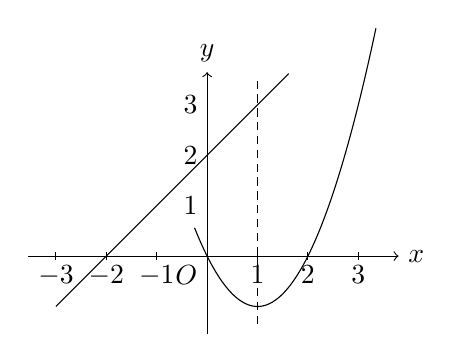
\begin{tikzpicture}[x=.64cm,y=.64cm,baseline=(current bounding box.center)]
  \draw[->] (-3.55,0)--(3.80,0) node[right] {$x$}; \draw[->] (0,-1.55)--(0,3.65) node[above] {$y$};
  \draw[domain=-.25:3.35,samples=100,smooth] plot (\x,{(\x-1)^2-1});
  \draw (-3.0,-1.0)--(1.62,3.62); \draw[densely dashed] (1,-1.35)--(1,3.55);
  \foreach \v in {-3,-2,-1,1,2,3} {\draw (\v,.08)--(\v,-.08); \node[below] at (\v,0) {$\v$};}
  \node[left] at (0,1) {$1$}; \node[left] at (0,2) {$2$}; \node[left] at (0,3) {$3$}; \node[below left] at (0,0) {$O$};
\end{tikzpicture}
